\documentclass{article}

\usepackage[utf8]{inputenc}

\usepackage{amsmath, bm}
\usepackage{graphicx}
\usepackage{amssymb}
\usepackage{float}
\usepackage{caption}
\usepackage{subcaption}
\usepackage{hyperref}
\usepackage{tikz}
\usepackage{layout}

\usepackage[margin=1in]{geometry}
\usepackage{listings}
\usepackage{xcolor}
\usepackage{color, colortbl}
\usepackage{textgreek}
\usepackage{mathrsfs}
\usepackage{savetrees}

\usepackage{titlesec}

\titleformat{\subsubsection}
  {\normalfont\selectfont}{\thesubsubsection}{1em}{}

\usetikzlibrary{calc}
\usetikzlibrary{angles,quotes} % for pic
\usetikzlibrary{patterns,snakes}
\usetikzlibrary{arrows}
\tikzset{>=latex} % for LaTeX arrow head

\setlength{\parskip}{\baselineskip}%
\setlength{\parindent}{0pt}%
\linespread{0.9}


\definecolor{codegreen}{rgb}{0,0.6,0}
\definecolor{codegray}{rgb}{0.5,0.5,0.5}
\definecolor{codepurple}{rgb}{0.58,0,0.82}
\definecolor{backcolour}{rgb}{0.95,0.95,0.92}

\lstdefinestyle{mystyle}{
    backgroundcolor=\color{backcolour},   
    commentstyle=\color{codegreen},
    keywordstyle=\color{magenta},
    numberstyle=\tiny\color{codegray},
    stringstyle=\color{codepurple},
    basicstyle=\ttfamily\footnotesize,
    breakatwhitespace=false,         
    breaklines=true,                 
    captionpos=b,                    
    keepspaces=true,                 
    numbers=left,                    
    numbersep=5pt,                  
    showspaces=false,                
    showstringspaces=false,
    showtabs=false,                  
    tabsize=2
}

\lstset{style=mystyle}



\begin{document}

\title{}
\author{lwp26}
\date{January 2025}
\maketitle

\section{Introduction}

The importance of the neutral point to the aircraft stability means that
it needs to be measured in flight tests.
However this cannot be done directly ...

\section{Results}

\subsection{Longitudinal Static Stability}
\subsubsection{Stick fixed neutral point}

Definition of the neutral point
\begin{equation}
    \frac{\partial C_w}{\partial \alpha} = - \frac{x_n}{c} \frac{dC_L}{d \alpha}
\end{equation}

\begin{figure}[H]
    \centering
    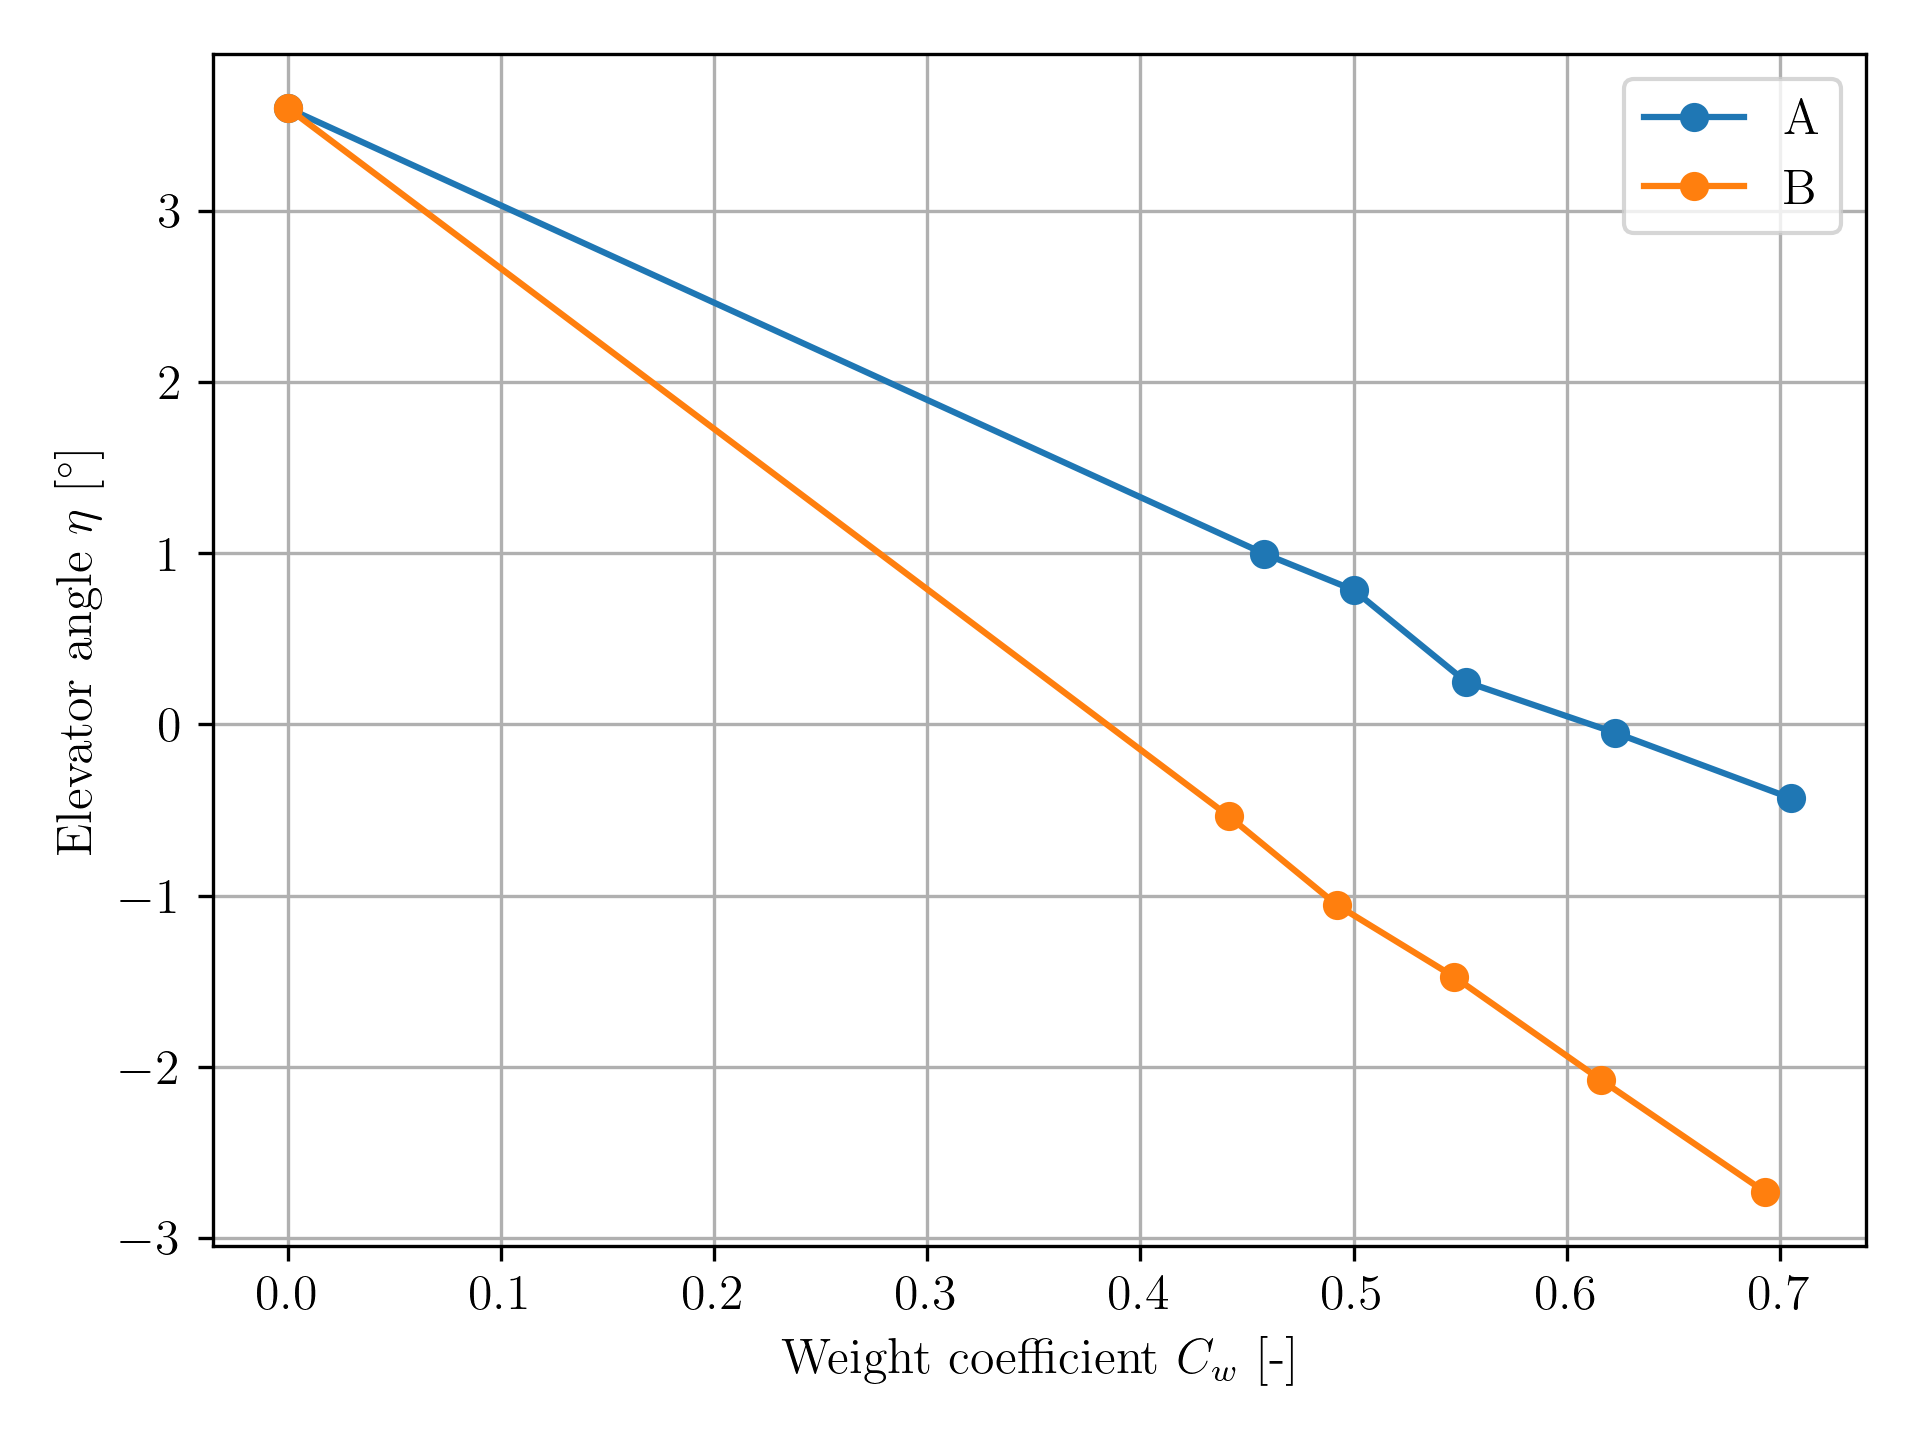
\includegraphics[width=0.8\textwidth]{Longitudinal_Static_Stability_1.png}
    \caption{}
    \label{fig:Longitudinal_Static_Stability_1}
\end{figure}
\begin{figure}[H]
    \centering
    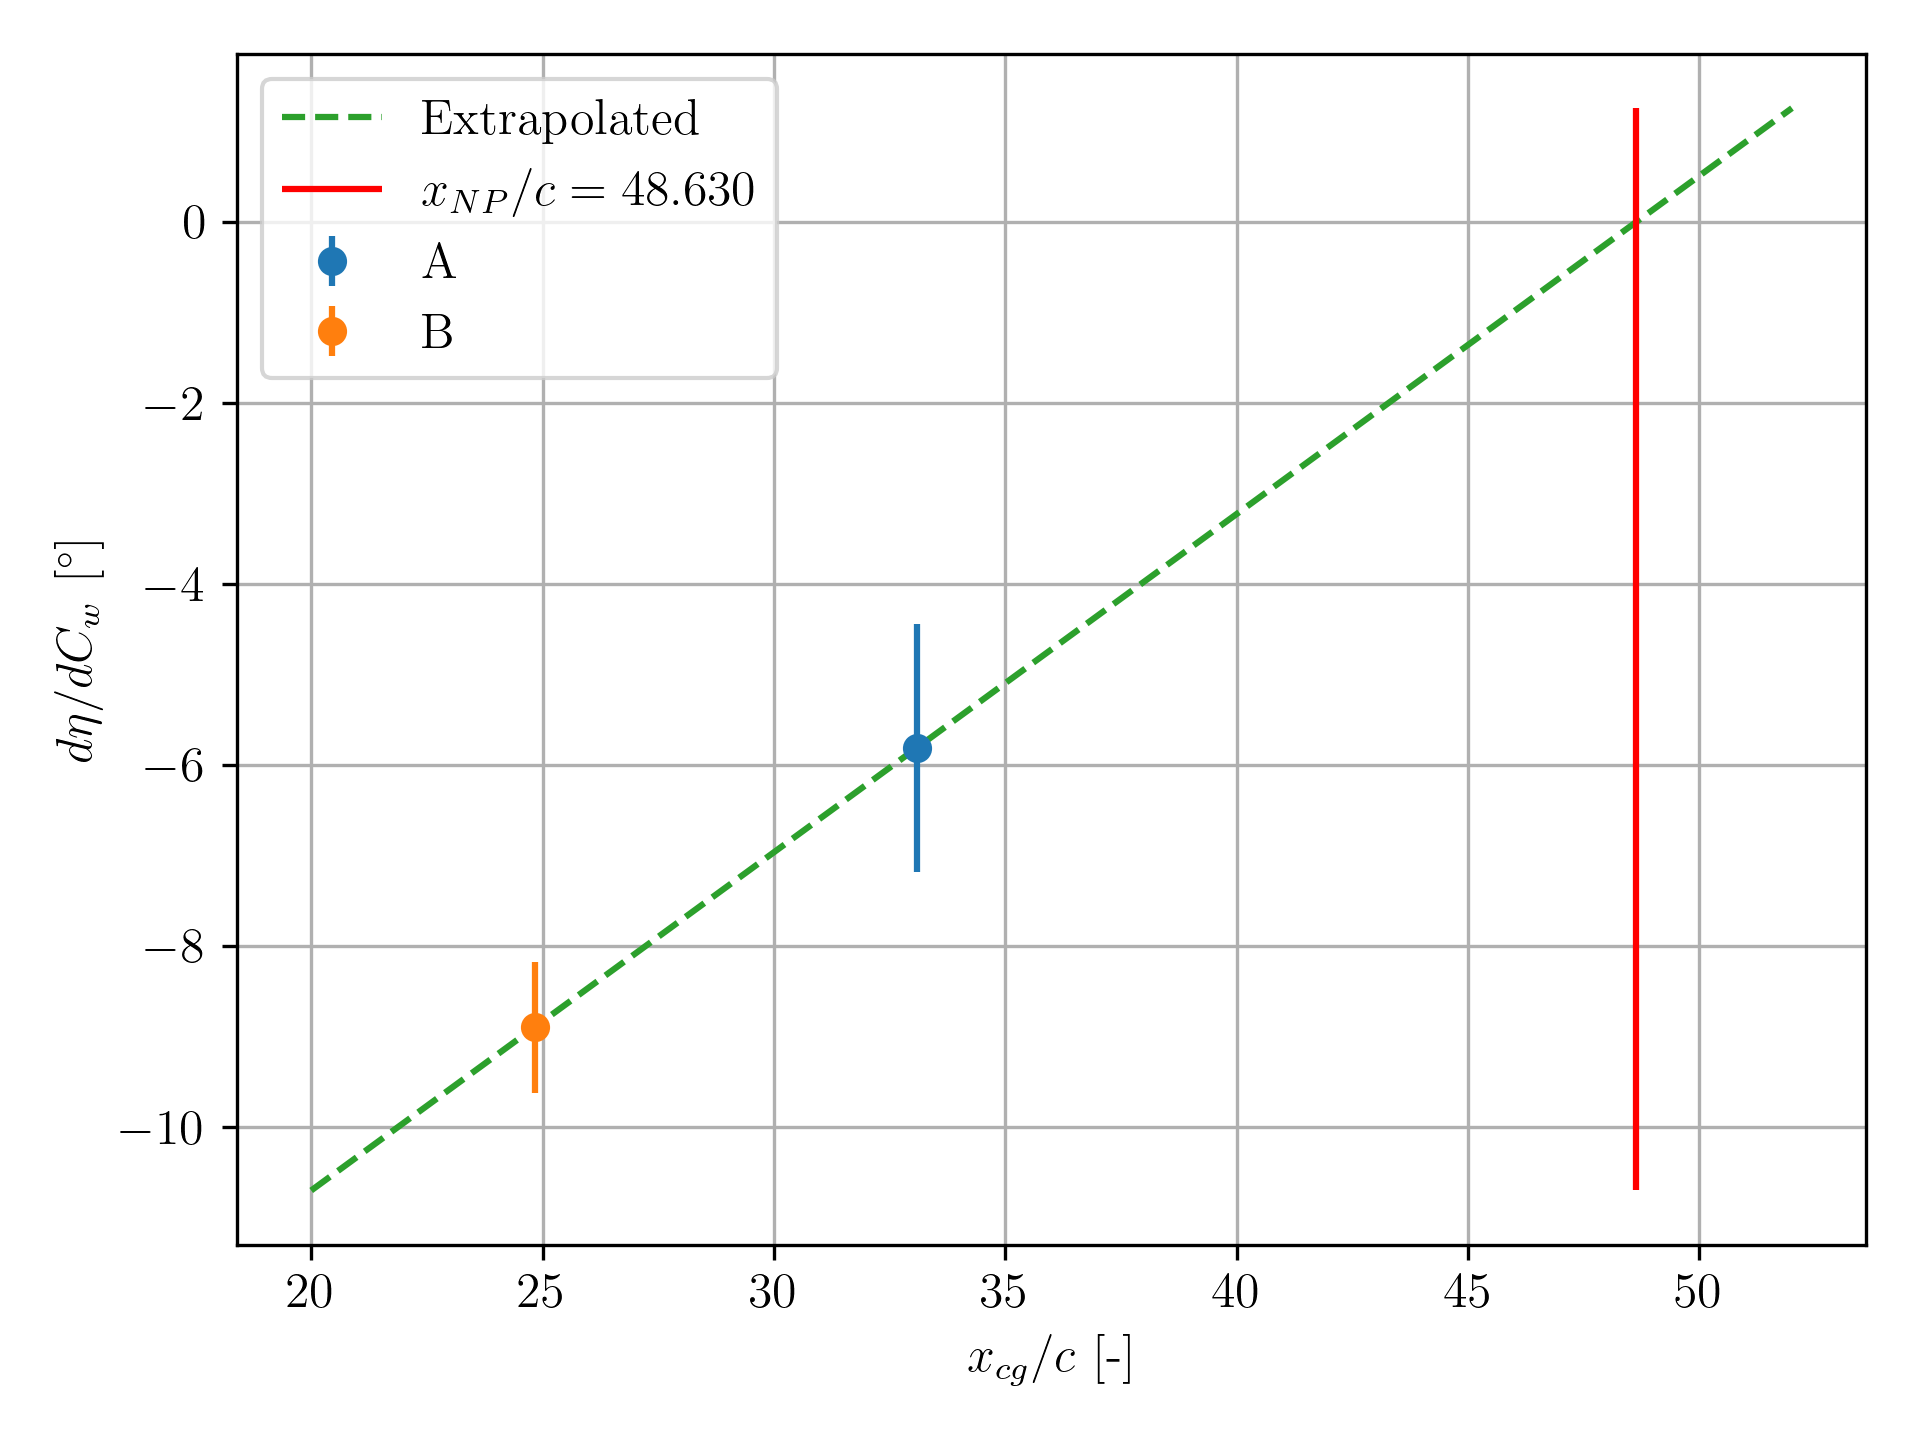
\includegraphics[width=0.8\textwidth]{Longitudinal_Static_Stability_2.png}
    \caption{}
    \label{fig:Longitudinal_Static_Stability_2}
\end{figure}

\subsubsection{Stick free neutral point}
\begin{figure}[H]
    \centering
    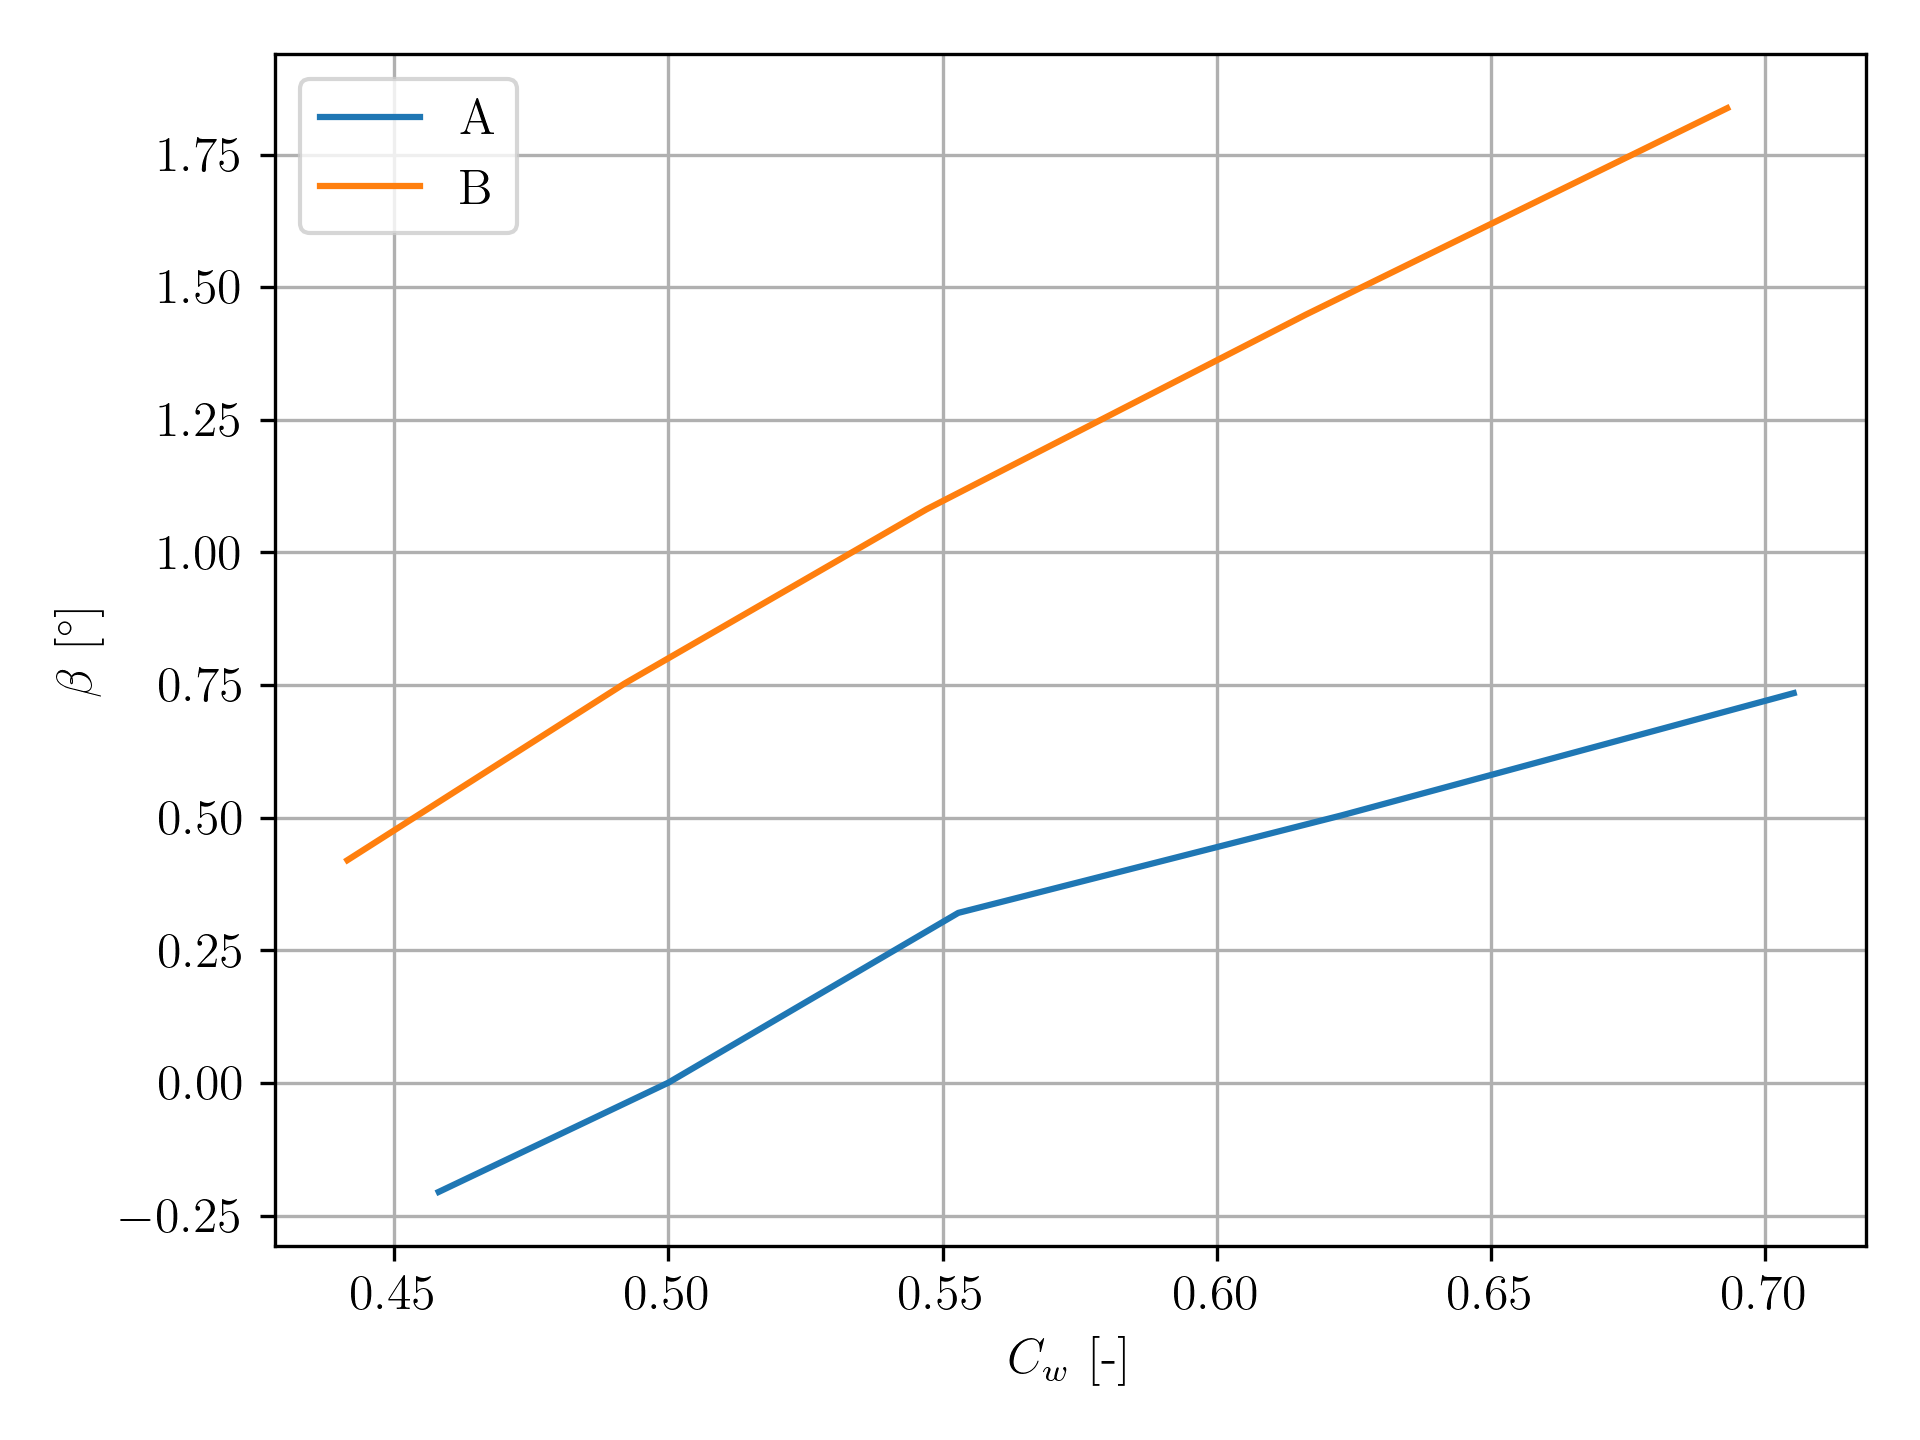
\includegraphics[width=0.8\textwidth]{Longitudinal_Static_Stability_3.png}
    \caption{}
    \label{fig:Longitudinal_Static_Stability_3}
\end{figure}
\begin{figure}[H]
    \centering
    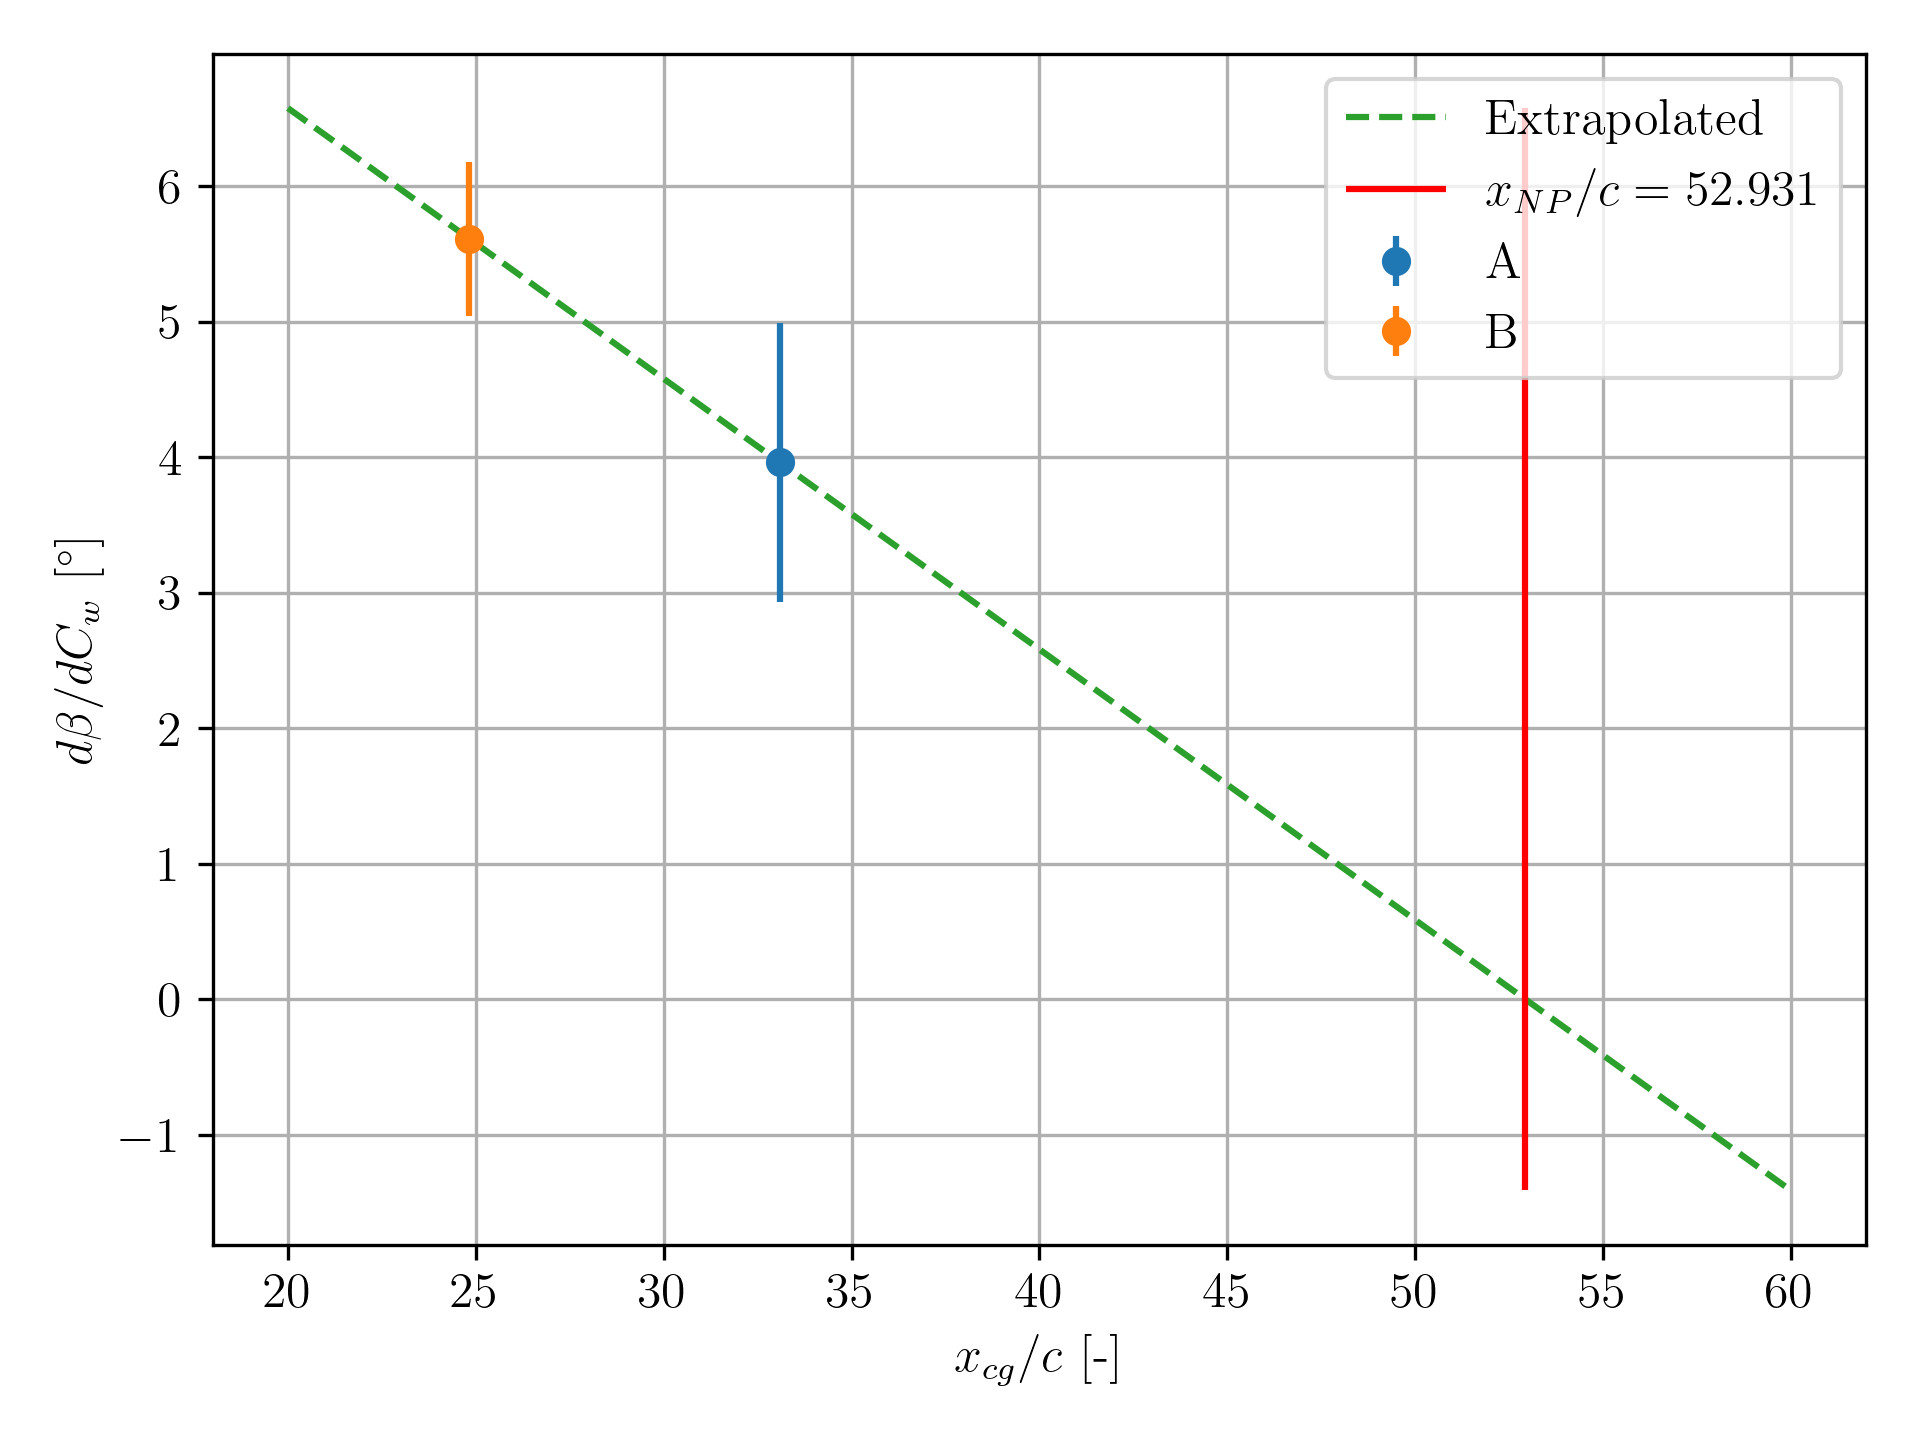
\includegraphics[width=0.8\textwidth]{Longitudinal_Static_Stability_4.png}
    \caption{}
    \label{fig:Longitudinal_Static_Stability_4}
\end{figure}

\subsection{Manoeuvre Stability}
\subsubsection{Stick fixed manoeuvre point}
\begin{figure}[H]
    \centering
    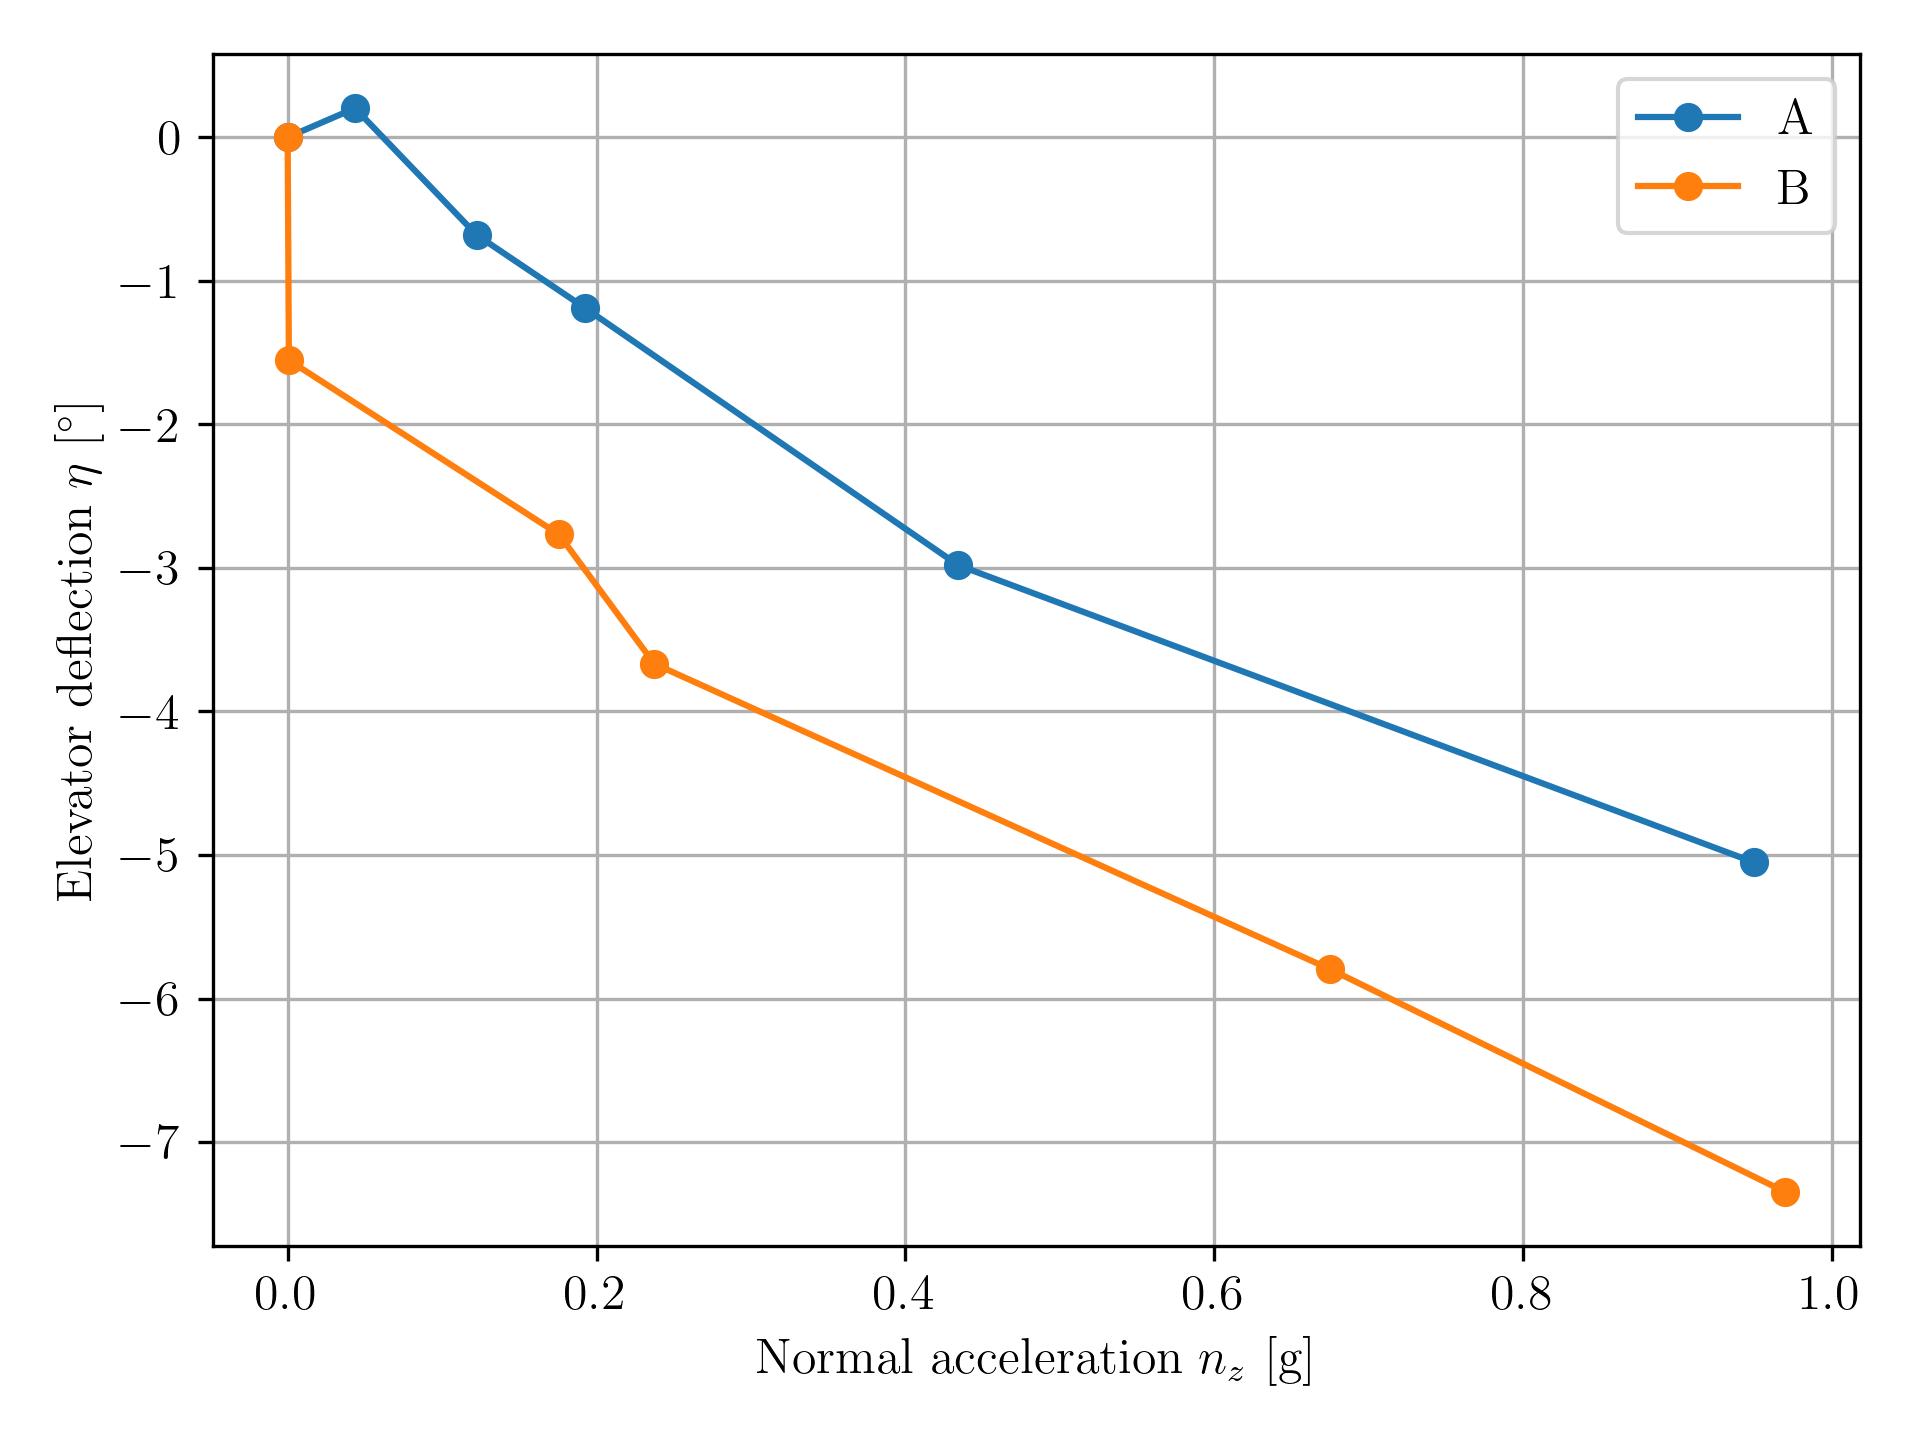
\includegraphics[width=0.8\textwidth]{Manoeuvre_Stability_1.png}
    \caption{}
    \label{fig:Manoeuvre_Stability_1}
\end{figure}
\begin{figure}[H]
    \centering
    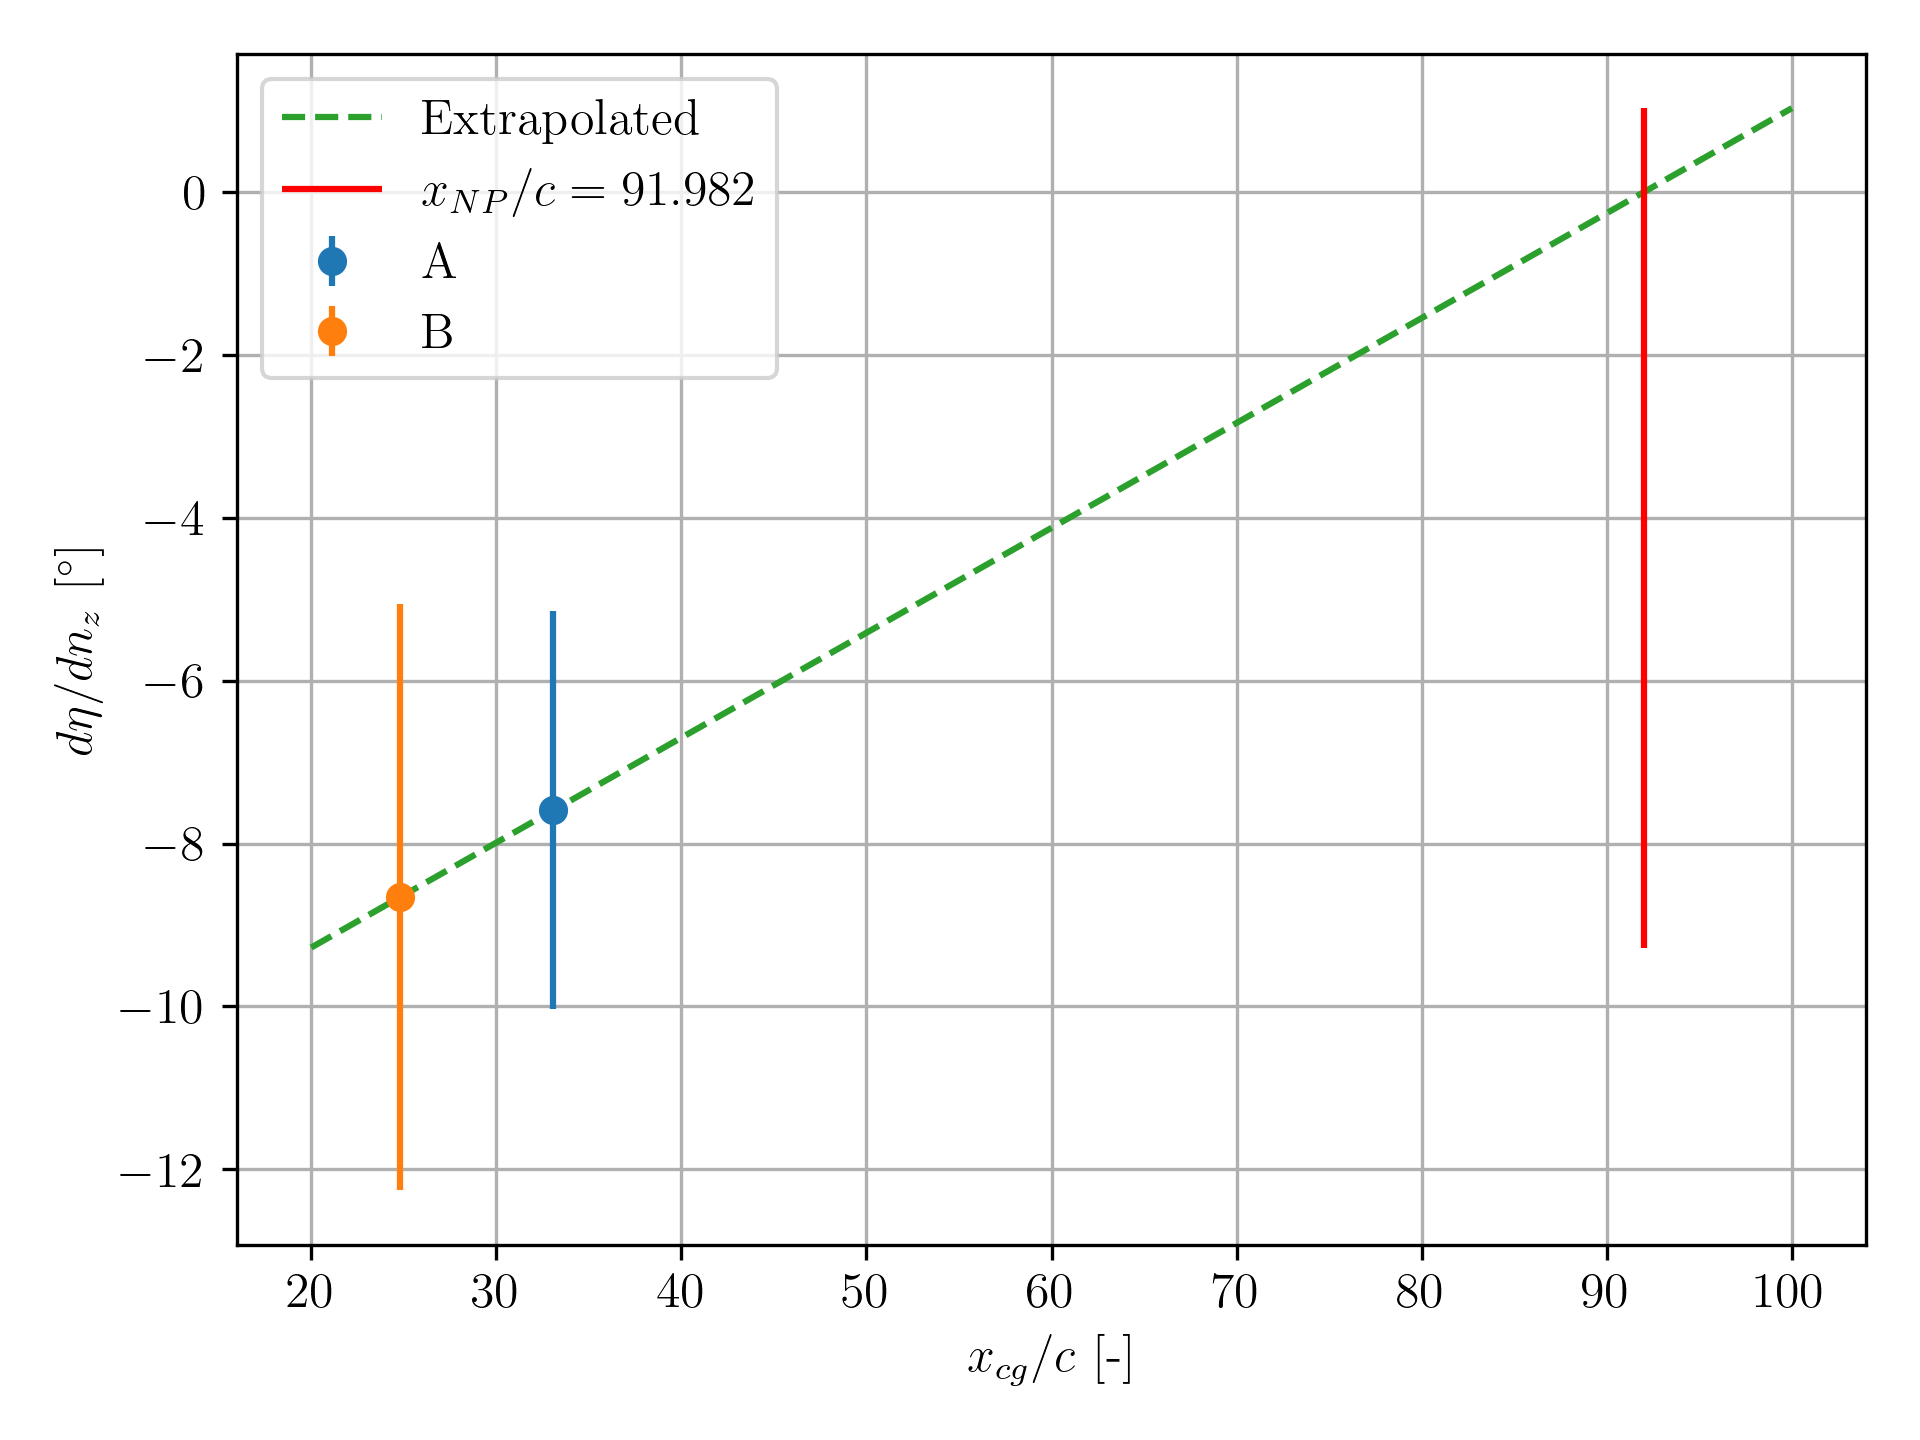
\includegraphics[width=0.8\textwidth]{Manoeuvre_Stability_2.png}
    \caption{}
    \label{fig:Manoeuvre_Stability_2}
\end{figure}
\subsubsection{Stick free manoeuvre point}
\begin{figure}[H]
    \centering
    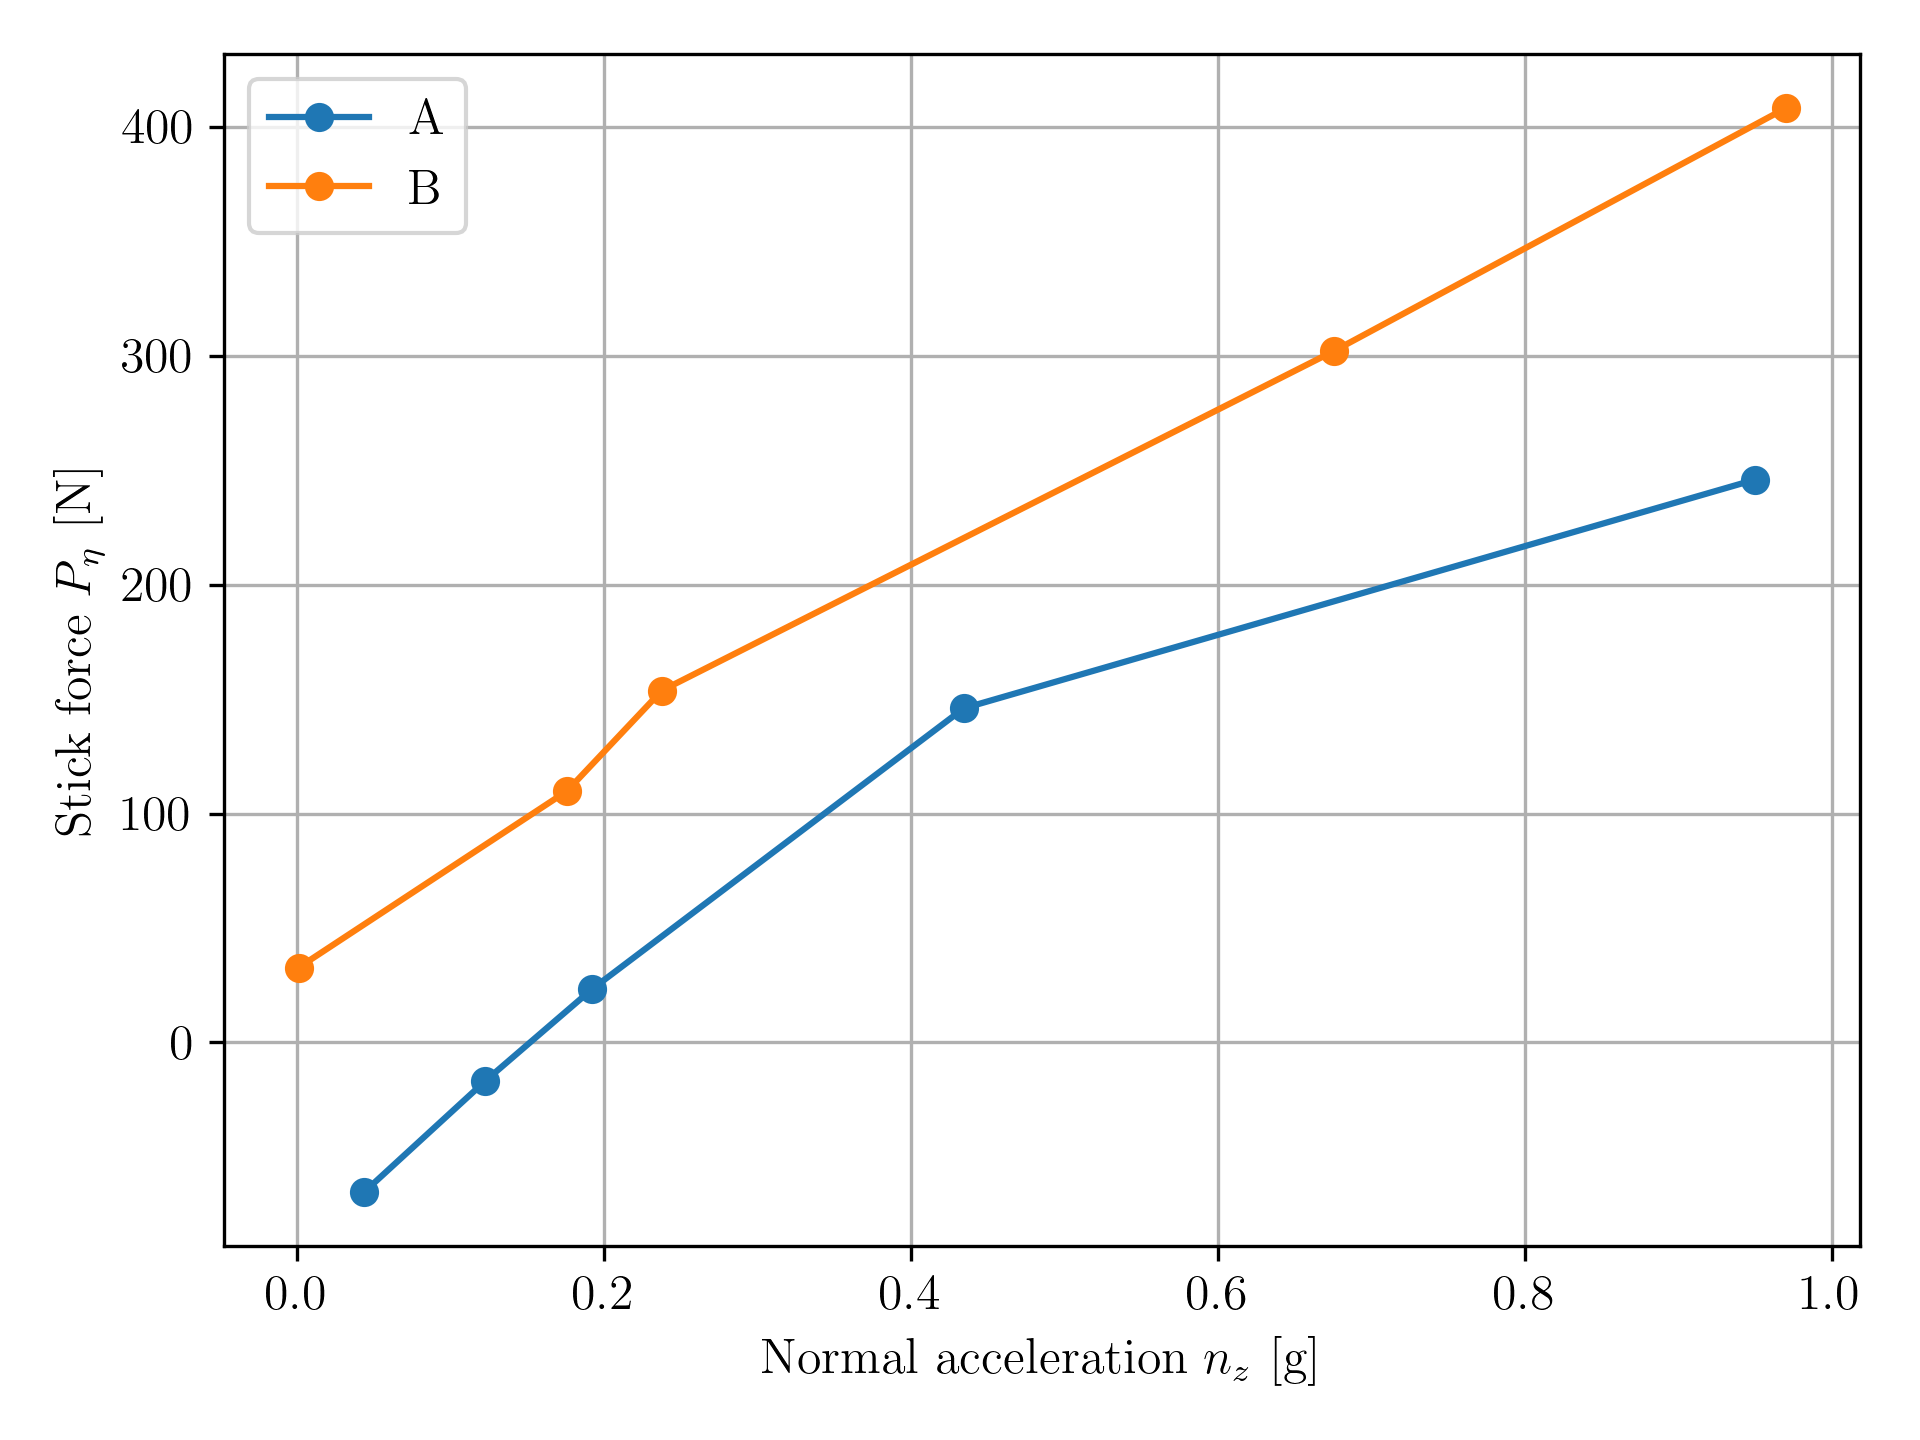
\includegraphics[width=0.8\textwidth]{Manoeuvre_Stability_3.png}
    \caption{}
    \label{fig:Manoeuvre_Stability_3}
\end{figure}
\begin{figure}[H]
    \centering
    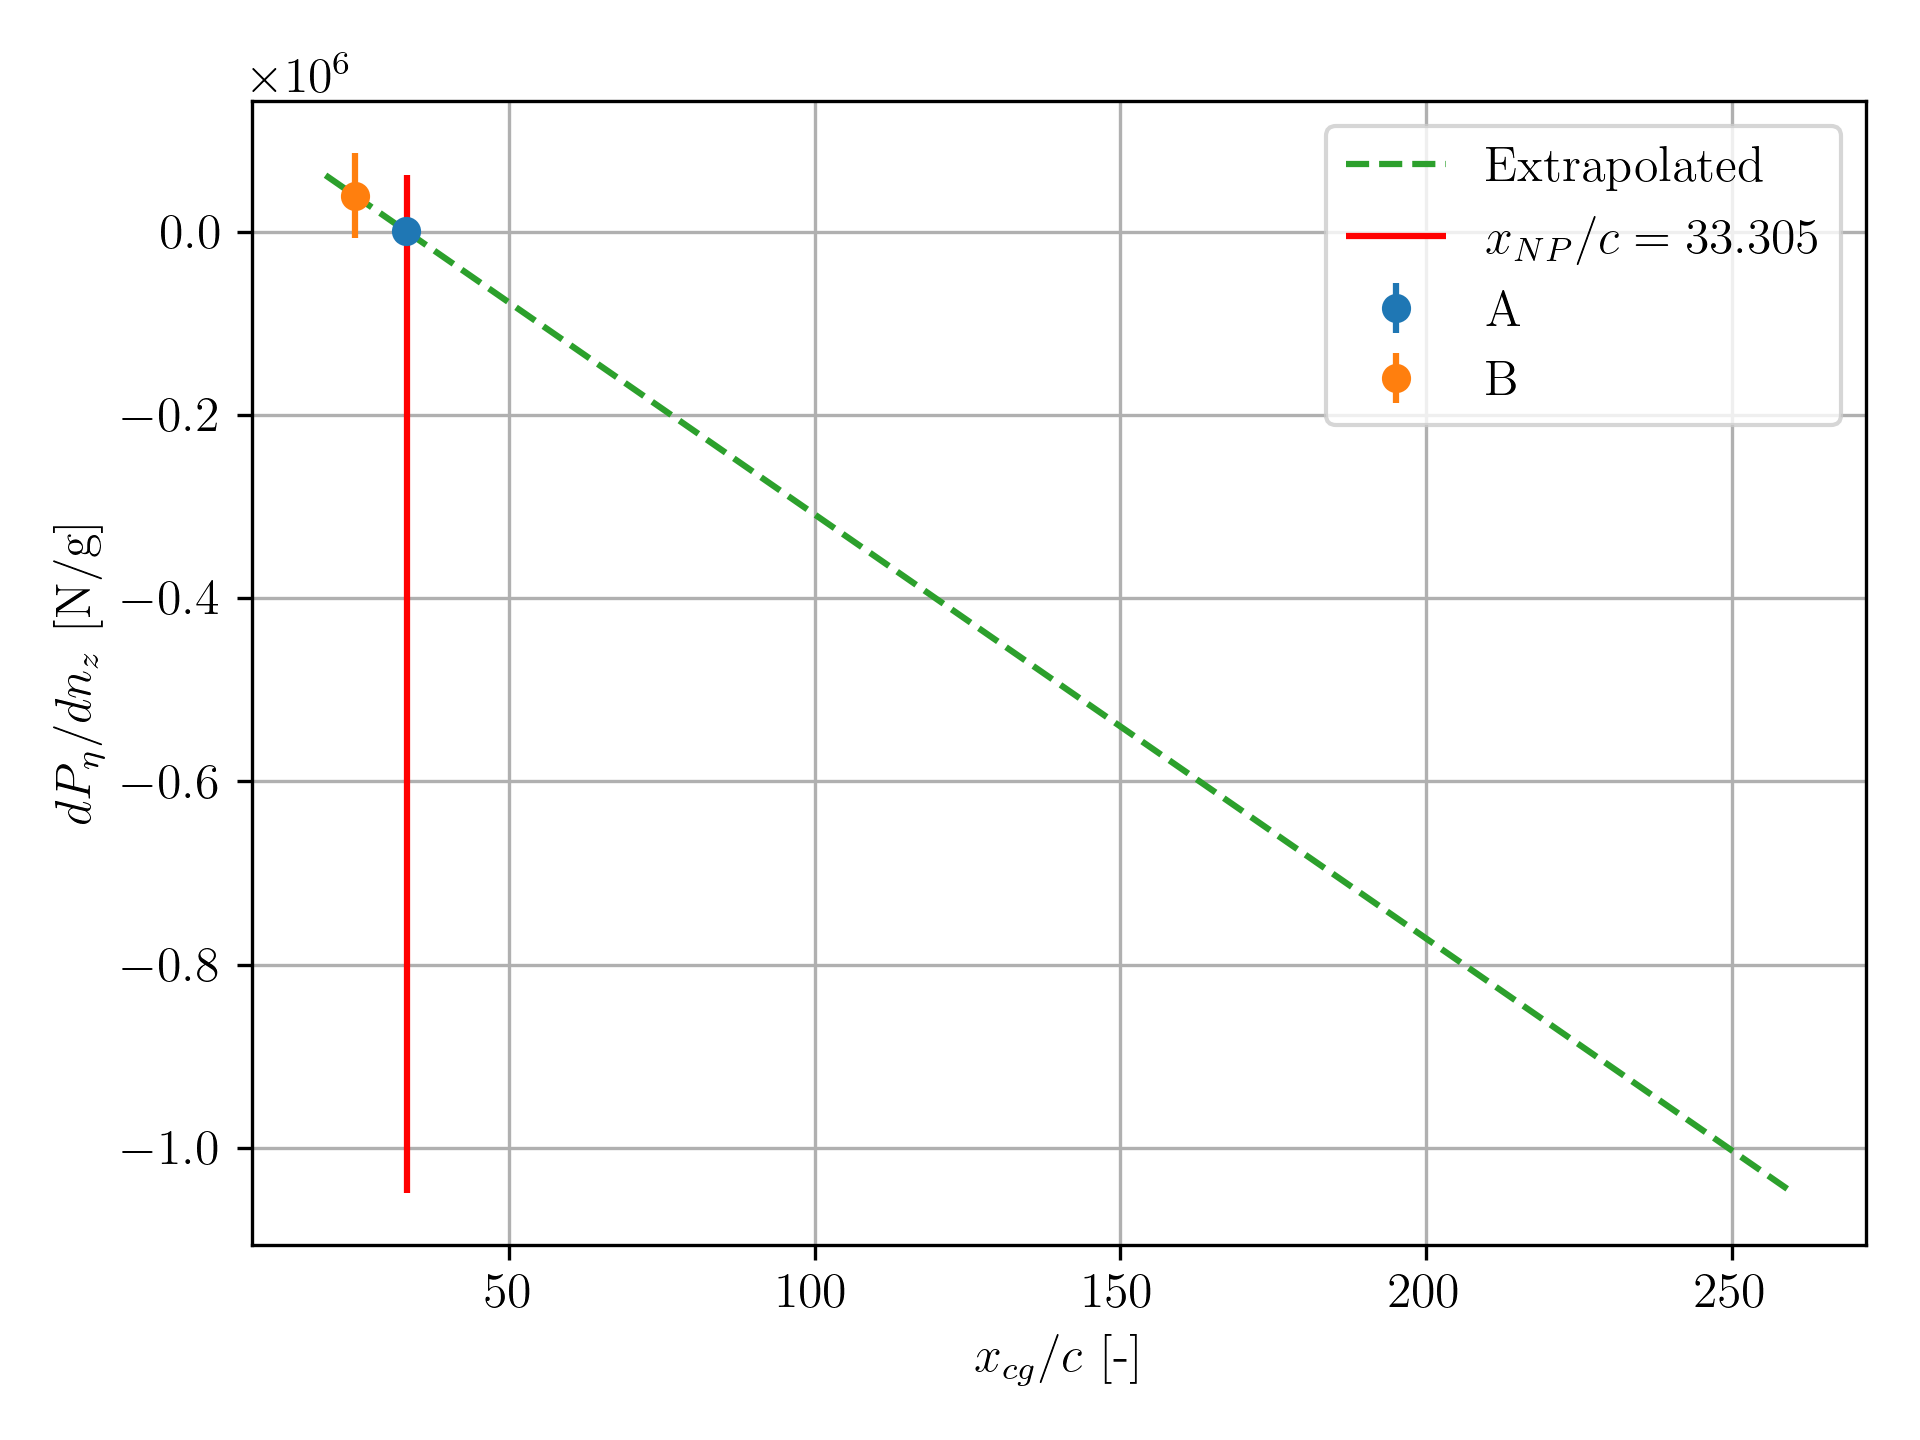
\includegraphics[width=0.8\textwidth]{Manoeuvre_Stability_4.png}
    \caption{}
    \label{fig:Manoeuvre_Stability_4}
\end{figure}

\subsection{Lateral-Directional Static Stability}

\begin{figure}[H]
    \centering
    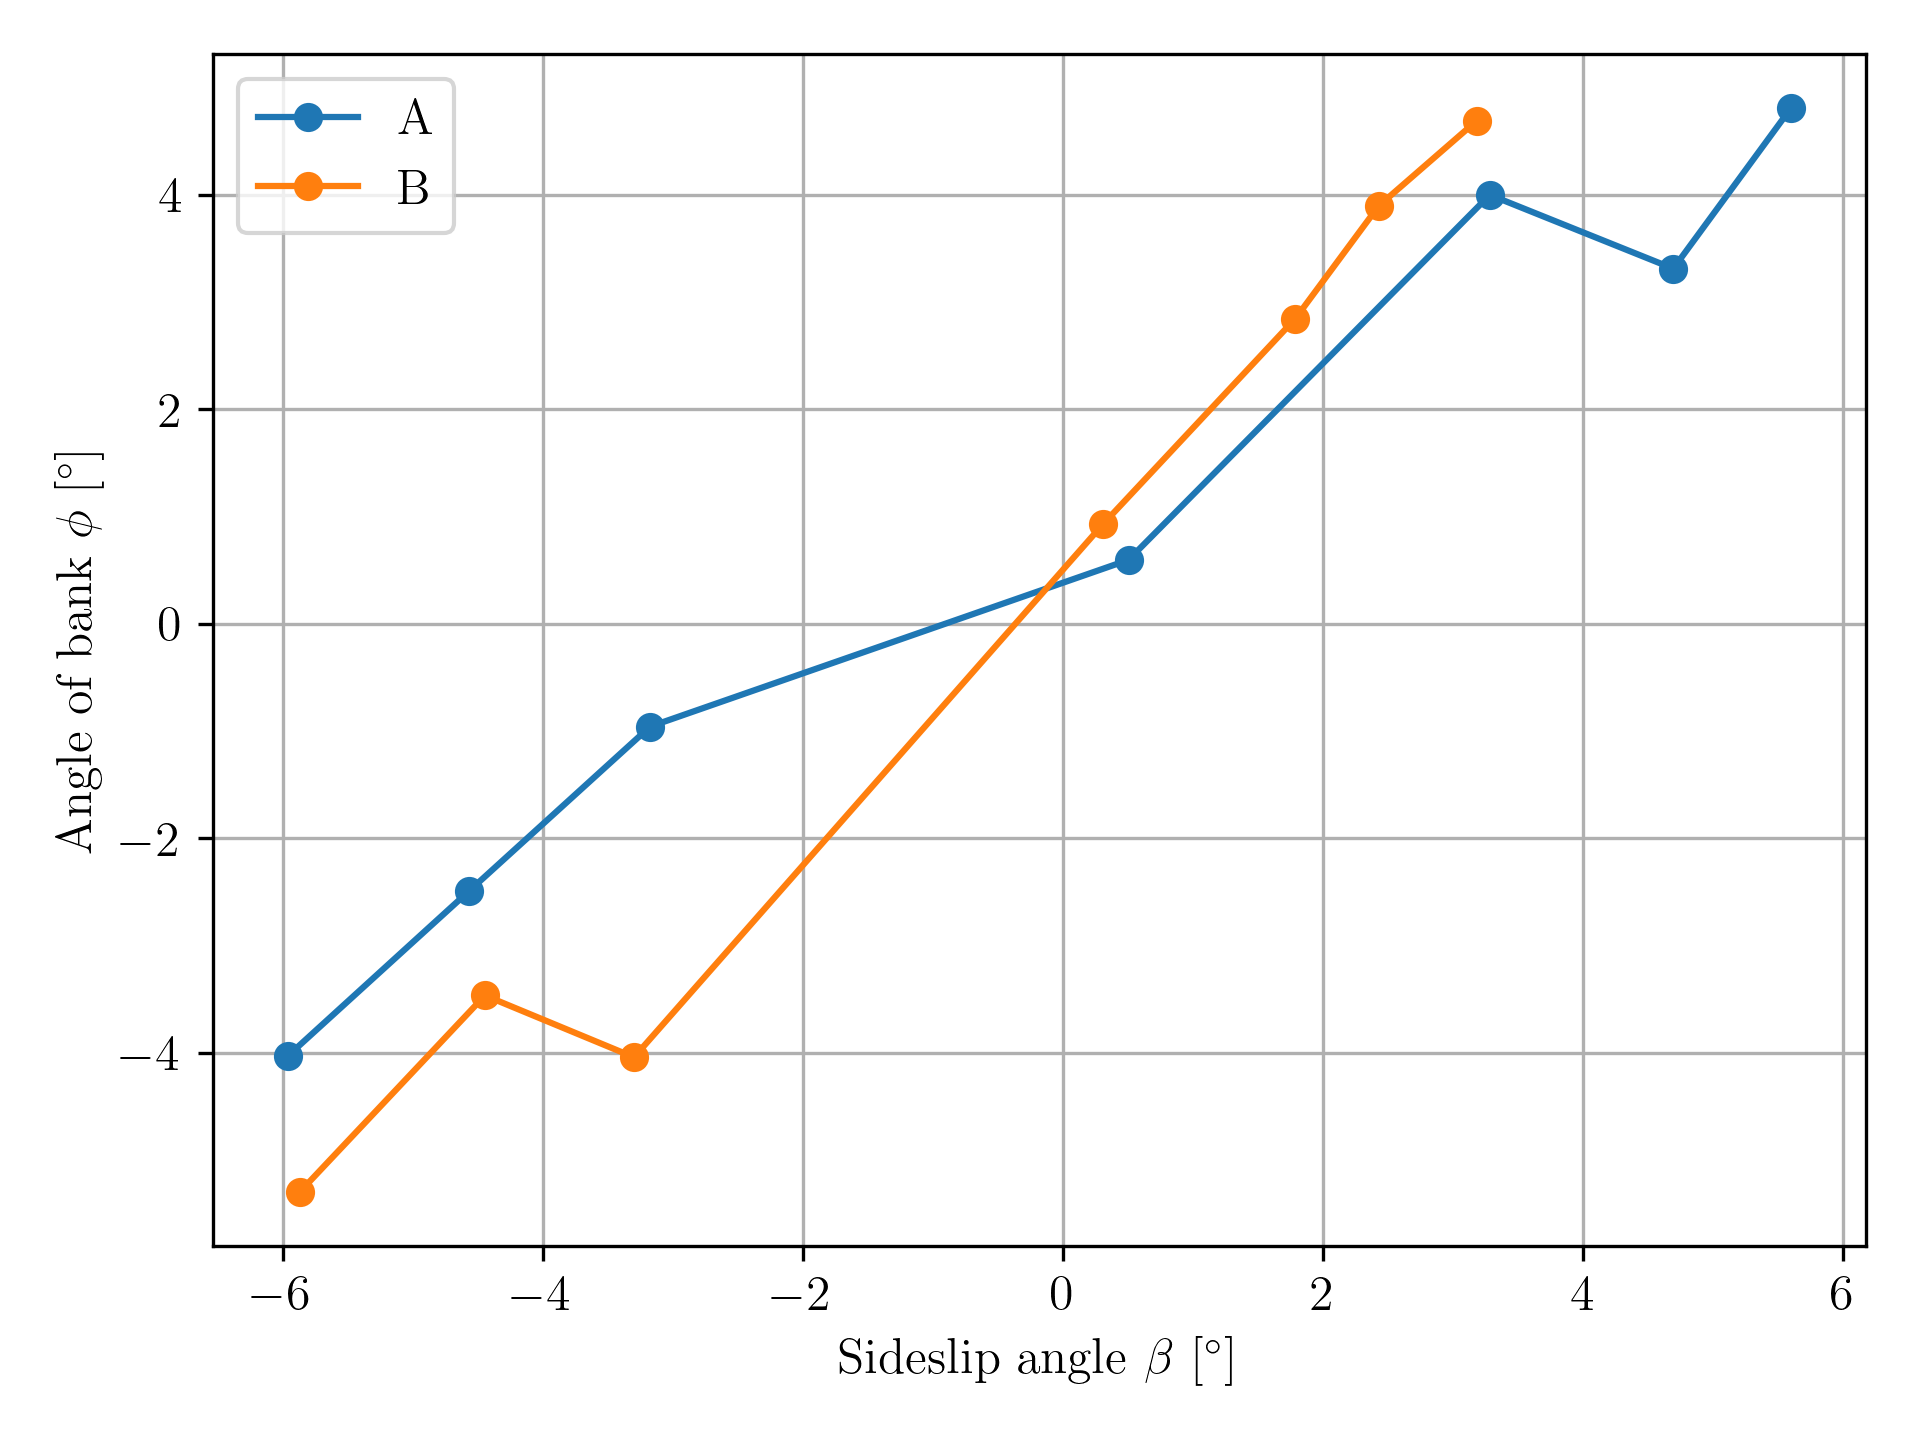
\includegraphics[width=0.8\textwidth]{Lat_Directional_Static_Stability_SHSS_1.png}
    \caption{}
    \label{fig:Lat_Directional_Static_Stability_SHSS_1}
\end{figure}

\subsubsection{Stick fixed lateral directional stability}
\begin{figure}[H]
    \centering
    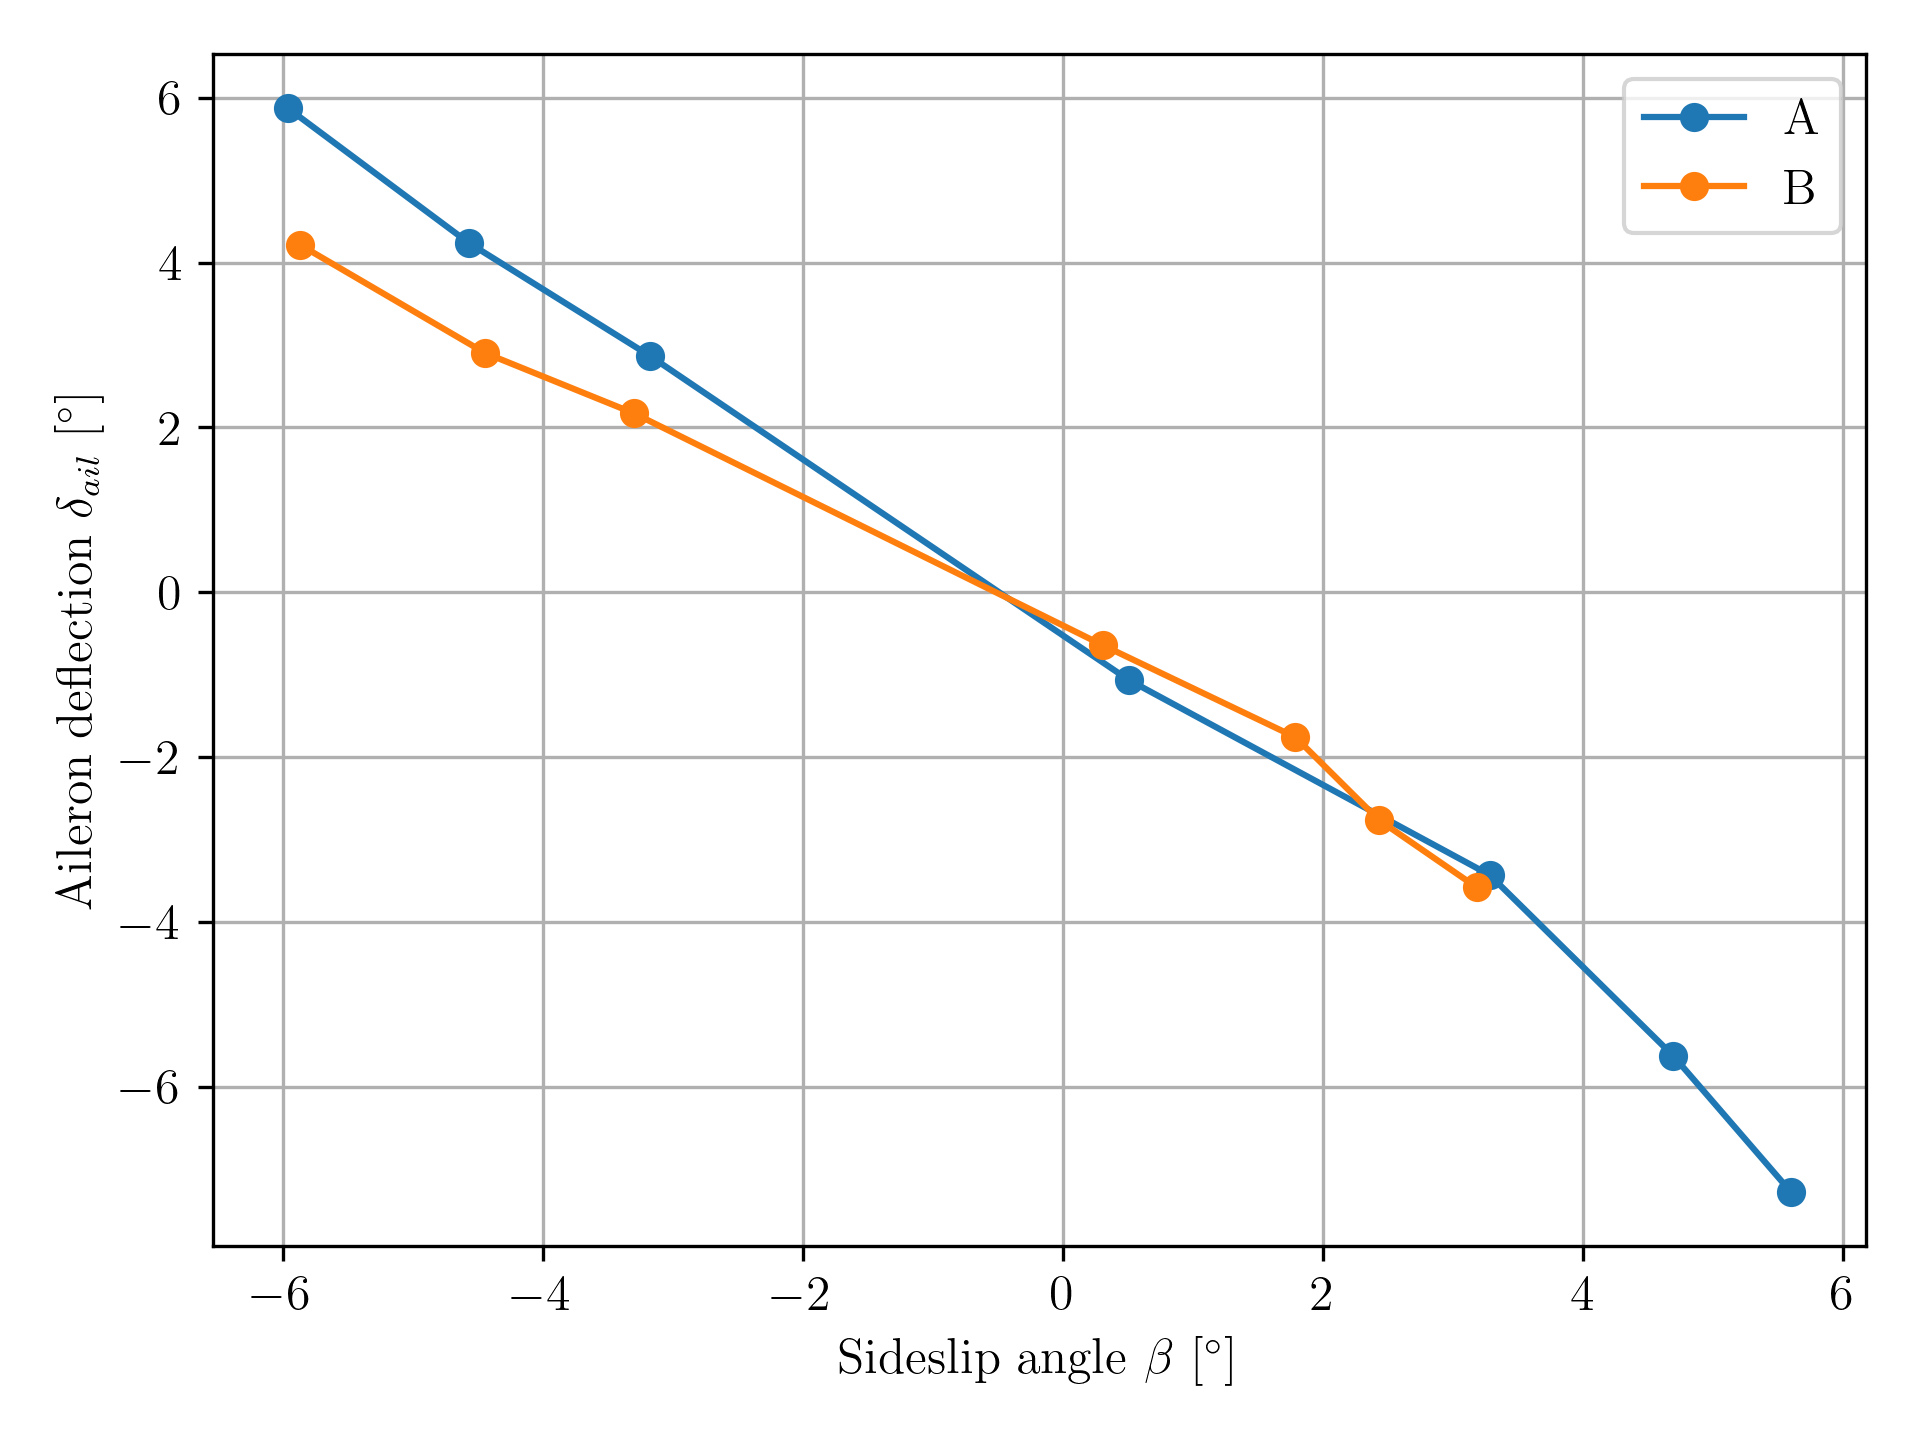
\includegraphics[width=0.8\textwidth]{Lat_Directional_Static_Stability_SHSS_2.png}
    \caption{}
    \label{fig:Lat_Directional_Static_Stability_SHSS_2}
\end{figure}

\begin{figure}[H]
    \centering
    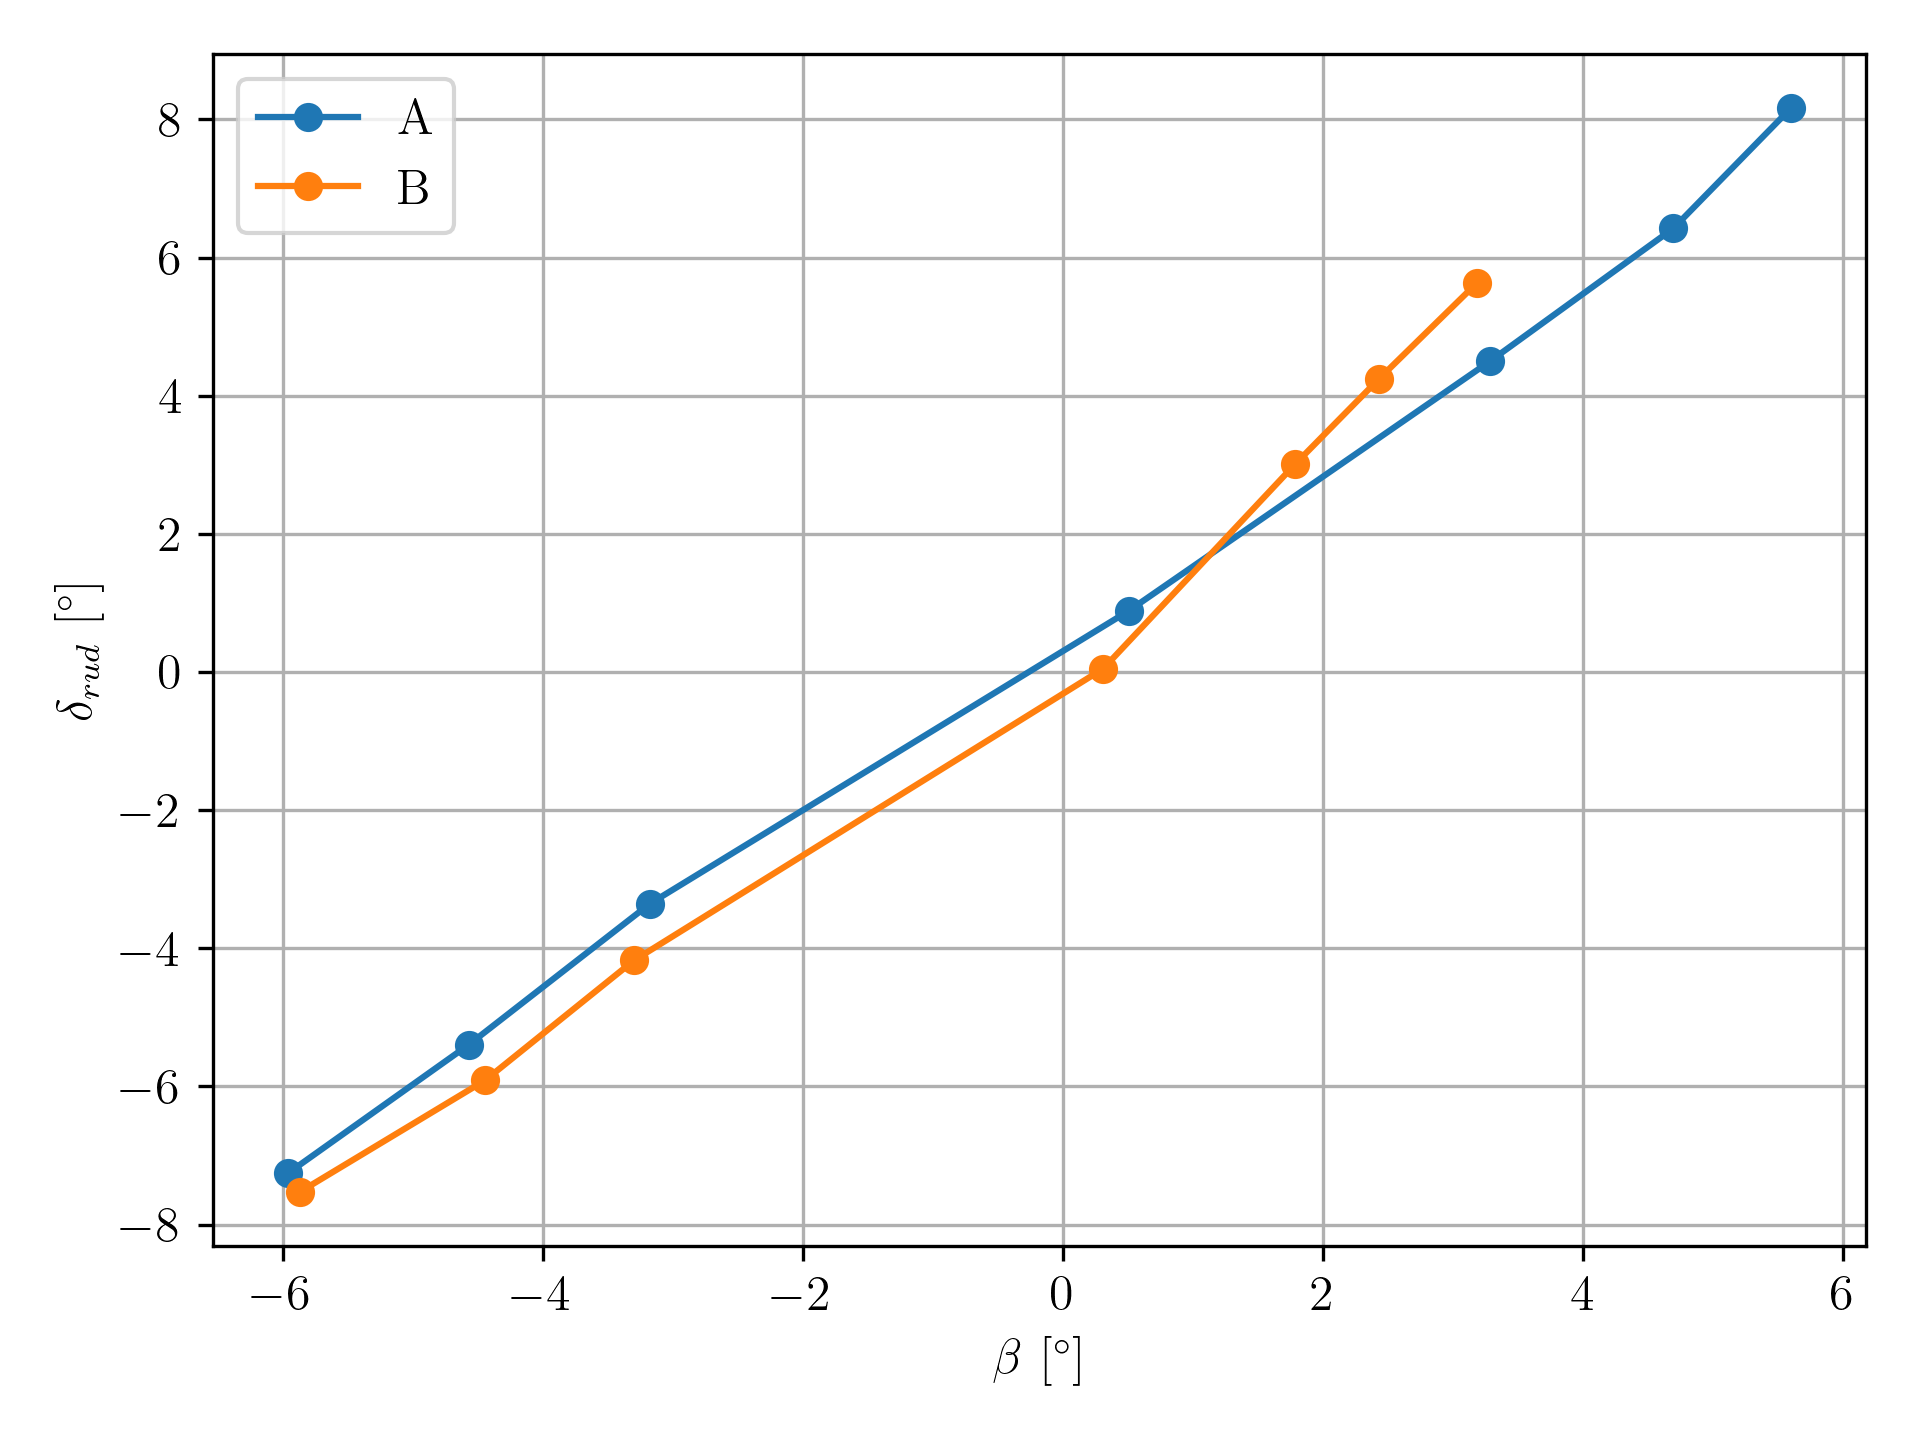
\includegraphics[width=0.8\textwidth]{Lat_Directional_Static_Stability_SHSS_3.png}
    \caption{}
    \label{fig:Lat_Directional_Static_Stability_SHSS_3}
\end{figure}


\begin{thebibliography}{9}

  \bibitem{handout}
  S. Place, A. Cooke
  \emph{Flight Experimental Methods: Course Handbook}
  Cranfield University,

\end{thebibliography}

\end{document}

